In this chapter, we would like to see how our results scales with the neutral density using our simple model for neutral collision of \cref{eq:elArColl}.
By fixing the magnetic $B$-field to $B_0=0.06\T$, we scan the degree of ionization $d$ in $80\%$, $60\%$, $40\%$, $20\%$, $1\%$, where $d$ is given by
%
\begin{align*}
    d = \frac{n_i}{n_i+n_n},
\end{align*}
%
where we take $n_i=n_0$ based on our quasi-neutral assumption.
This corresponds to neutral density values of
$2.5\cdot10^{18}\m^{-3}$,
$6.7\cdot10^{18}\m^{-3}$,
$1.5\cdot10^{19}\m^{-3}$,
$4.0\cdot10^{19}\m^{-3}$ and
$9.9\cdot10^{20}\m^{-3}$
respectively.
In experiments, ionization degrees from $0.1\%$ up to $100\%$ has been observed \cite{Schroder2003Phd}.

With our parameters, the neutral collisions ranges from $\nu_{en}=1.87\cdot10^{5}\s^{-1}$ at $d=80\%$, and scales linearly with $n_n$ up until $d=1\%$, where $\nu_{en}=7.38\cdot10^7\s^{-1}$.
The electron-ion collision frequency is $\nu_{ei}=7.25\cdot10^7 \s^{-1}$ throughout the scan range, meaning that the neutral collisions will dominate firstly only at $d=1\%$.

To keep the model consistent, $\nu_{in}$ will be kept to zero as $T_i=0$.
The physical justification for this is questionable as we assume that ions are streaming against stationary ions (see \cref{app:collisions} for details).
However, if all the ions are misaligned with respect to the neutrals, no collision will take place.
In any case, we usually have $\nu_{in}\ll\nu_{en}$ \cite{Schroder2003Phd}, which means that the $\nu_{in}$ term in \cref{eq:celma_vortD_evolution} is negligible.

\section{The steady state}

Starting with the parallel profiles shown in \cref{fig:nnScanPar}, we can note that the profiles remains constant until $d=1\%$.
%
\begin{figure}[htb]
    \centering
    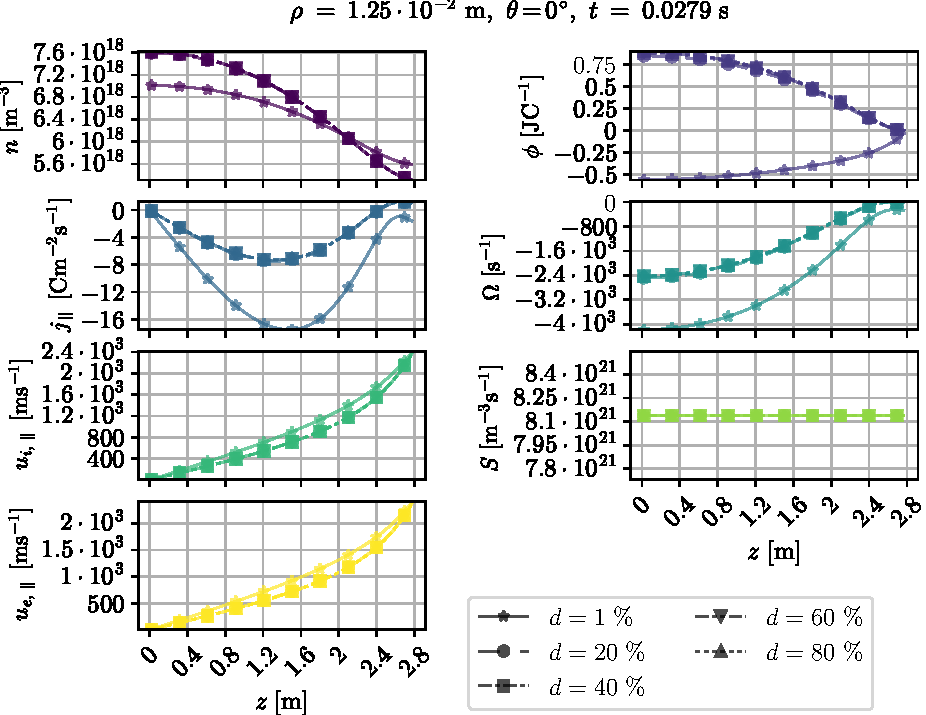
\includegraphics{fig/results/neutral/nnScanPar}
    \caption{The parallel steady state profiles as a function of $d$.}
    \label{fig:nnScanPar}
\end{figure}
%
At $d=1\%$ the peak density drops with almost $10\%$, and the parallel profiles flattens.
More importantly, the system no longer follows the Boltzmann response.
In fact, $n$ and $\phi$ now behaves inversely.
For high $n$, the potential is low and vice versa.
As explained in \cref{chap:ss}, there is a tight connection between $\phi$, $j_\|$ and $\Om$.
If one of them changes, the rest follows.
We recall that $\phi$ is not evolved in time like $n$, but is entirely determined by the \emph{radial} profile of $\Om^D$ in each parallel point.
Therefore, we will explain the change in the parallel profiles by explaining the radial profiles.

The radial profiles are shown in \cref{fig:nnScanRad}.
%
\begin{figure}[htb]
    \centering
    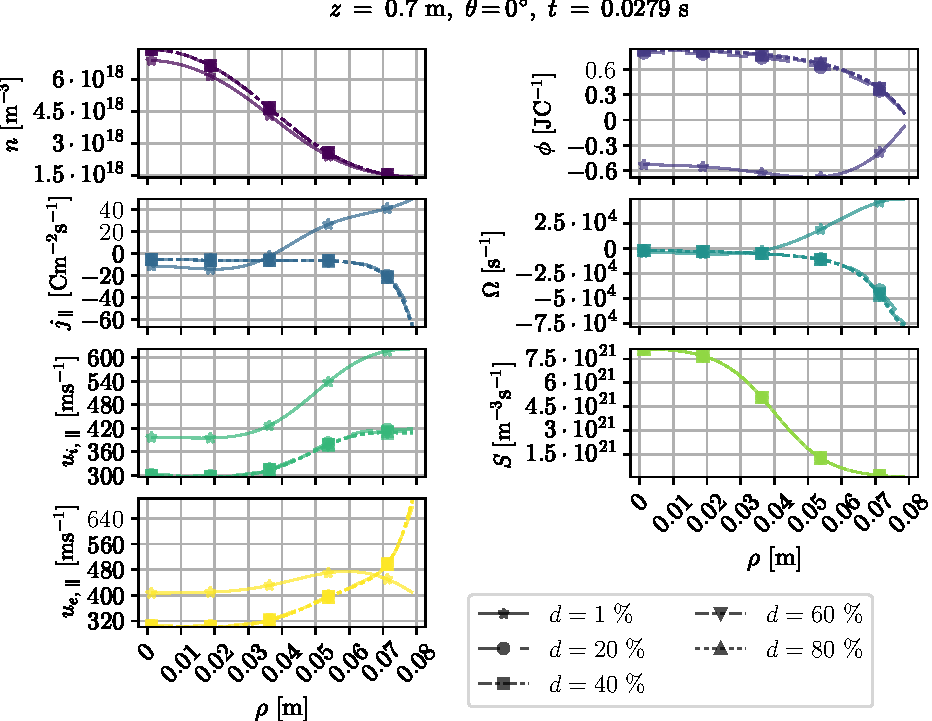
\includegraphics{fig/results/neutral/nnScanRad}
    \caption{The radial steady state profiles as a function of $d$.}
    \label{fig:nnScanRad}
\end{figure}
%
In terms of the density, there is a minimal change in the profile when the ionization degree is changed.
The potential, on the other hand, has changed sign, and is negative for all the radii until the boundary condition, which is set at $0$.
This can be explained from the $\Om$-profile which for $d=1\%$ takes higher values for increasing $\rho$, which is opposite of the other ionization degrees.
To explain this behavior, we must look at the balancing terms of the modified vorticity, which is shown in \cref{fig:nnScanVortDRad}.
%
\begin{figure}[h!]
    \centering
    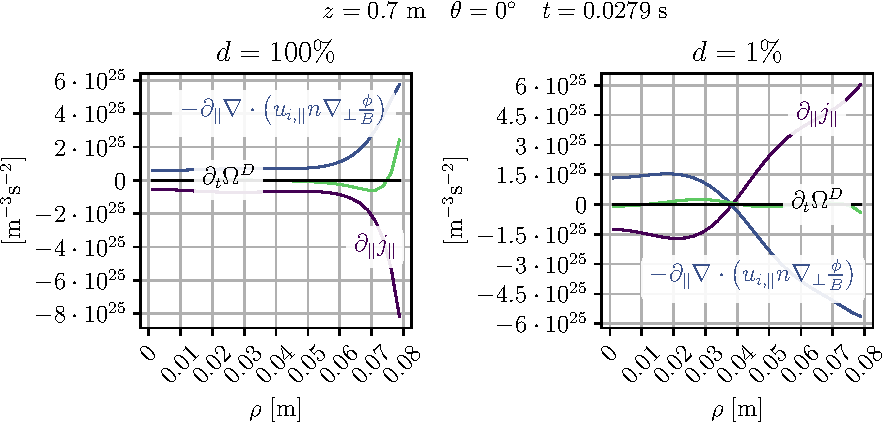
\includegraphics{fig/results/neutral/vortDBalanceNnCompareRad}
    \caption{The radial steady state balance for the modified vorticity for $d=100\%$ and $d=1\%$.
        The green, unlabeled line denotes the artificial vorticity.
    }
    \label{fig:nnScanVortDRad}
\end{figure}
%
In the fully ionized plasma the time change of the modified vorticity is kept to zero as the parallel derivate of the current is balancing the parallel derivative of the ion velocity multiplied modified vorticity.
This same terms accounts for the balance in the $d=1\%$ case.
However, in the $d=1\%$ case, the profiles crosses zero and behaves opposite for high $\rho$ than what is observed for the $d=100\%$ case.
As $\Om^D$ does not contain any $\nu_{en}$ terms, we will explain this behavior by looking into the balancing terms for the parallel current displayed in \cref{fig:nnScanJParRad}.
%
\begin{figure}[htb]
    \centering
    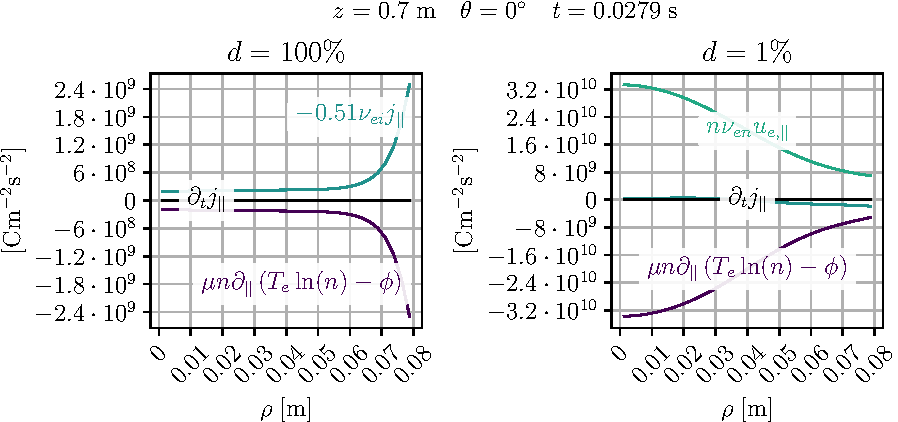
\includegraphics{fig/results/neutral/jParBalanceNnCompareRad}
    \caption{The radial steady state balance for the parallel current for $d=100\%$ and $d=1\%$.}
    \label{fig:nnScanJParRad}
\end{figure}
%
In the $d=100\%$ case the Boltzmann term is balanced by the electron-ion resistivity.
On the other hand, for $d=1\%$ the electron-neutral term is dominating the electron-ion resistivity term by one order magnitude.
As a consequence, the resulting $j_\|$ profile must change.
Since the $j_\|$ profile changes, the $\Om^D$ balance changes, and the $\phi$ profile changes.
As $\phi$ changes, the Boltzmann term changes, which again changes the $j_\|$.
From this feed-back loop the vorticity profile changes in the radial direction.

We can now return to the initial question on why the parallel profiles changes.
Recall that the parallel potential profile is determined by the perpendicular vorticity plane.
The radial modified vorticity profiles are shown in \cref{fig:nnScanVortDPar}.
%
\begin{figure}[htb]
    \centering
    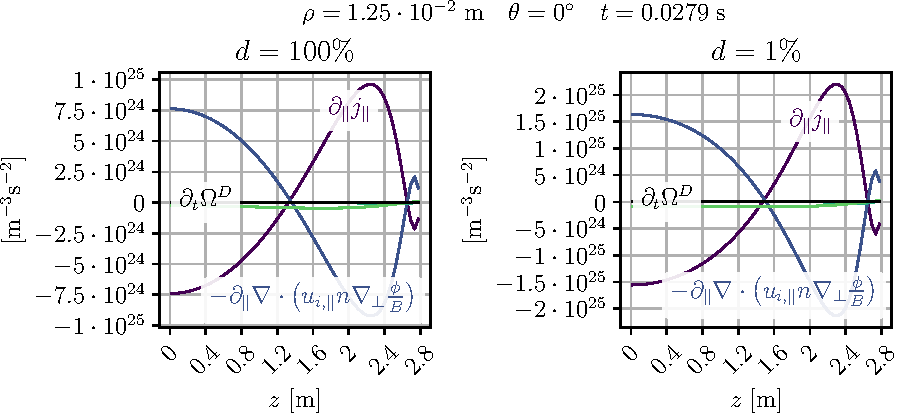
\includegraphics{fig/results/neutral/vortDBalanceNnComparePar}
    \caption{Parallel profiles of the modified vorticity balance.}
    \label{fig:nnScanVortDPar}
\end{figure}
%
We observe that although the profiles differs in value, the shapes of the balance remains the same.
This explains why the shape of the vorticity profiles in \cref{fig:nnScanPar} remains the same, only differing in values.
The parallel change of the radial profiles is just modified by the parallel current profiles, which is shown in \cref{fig:nnScanJParPar}.
%
\begin{figure}[htb]
    \centering
    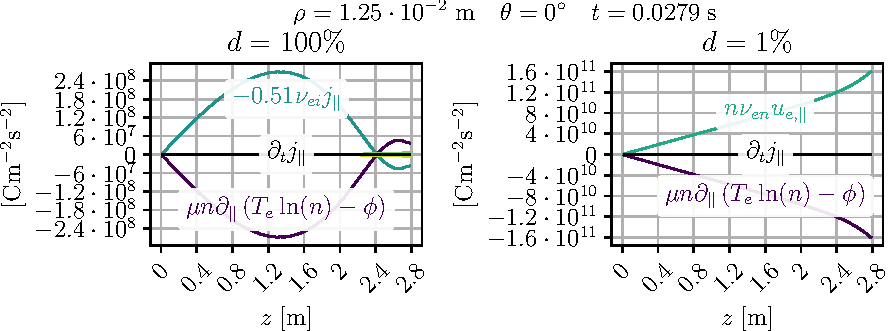
\includegraphics{fig/results/neutral/jParBalanceNnComparePar}
    \caption{Parallel profile of the parallel current.}
    \label{fig:nnScanJParPar}
\end{figure}
%
This determines the strength of the parallel current which is balancing the perpendicular vorticity.
As the perpendicular balance is changed, the parallel potential profile is changed.

\section{The linear phase}
%
We find the growth rates in the same manner as described in \cref{sec:grDesc}.
The result is presented in \cref{fig:grNnModeNr,fig:grNn}.
%
\begin{figure}[htbp]
    \centering
    \begin{subfigure}[h]{0.45\textwidth}
        \centering
        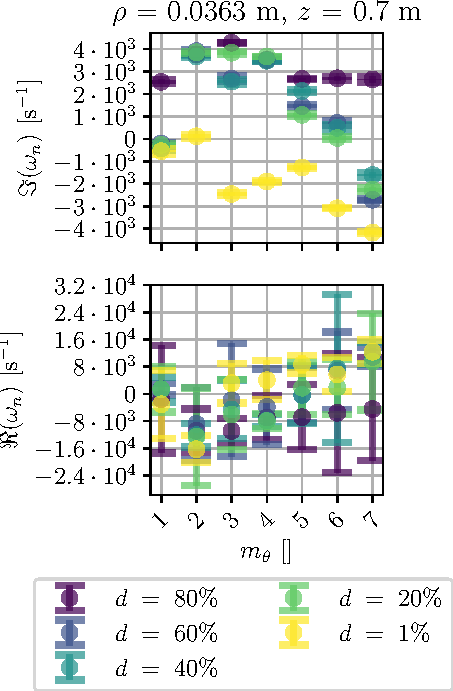
\includegraphics{fig/results/neutral/growthRatesNnScan}
        \caption{Growth rates and angular frequencies as a function of mode numbers.}
        \label{fig:grNn}
    \end{subfigure}%
    \hfill
    \begin{subfigure}[h]{0.45\textwidth}
       \centering
       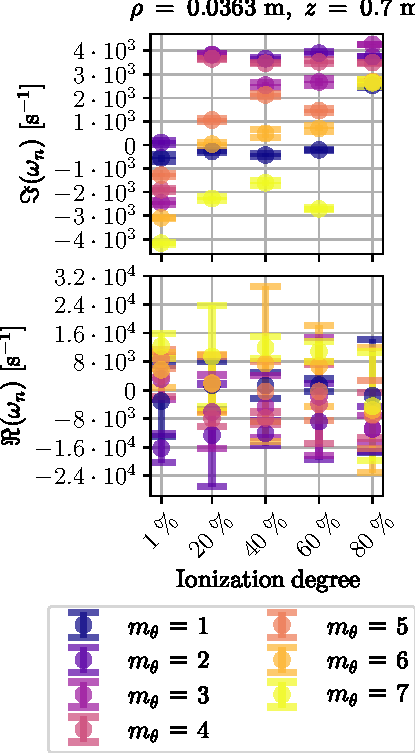
\includegraphics{fig/results/neutral/growthRatesNnModes}
       \caption{Growth rates and angular frequencies as a function of $d$}
       \label{fig:grNnModeNr}
    \end{subfigure}
\end{figure}
%
We observe that the general trend is that the growth rate decreases for decreasing ionization degree.
For higher mode numbers the rotation increases with decreasing $d$, whereas the converse is true for the low mode numbers.

The max growth rate is found around $m_\theta=2-3$.
As in the case with a fully ionized plasma, the decaying modes are rotating in the ion diamagnetic direction.
Of the growing modes, we can observe that there is less rotation for higher modes, with exception of the first mode, which is unstable for all the ionization levels with exception of $d=80\%$.
Finally, we note that $d=1\%$ is only slightly unstable.

This low ionization level is also the only one which does not reach a saturated steady state, but rather saturates in a situation where the modes are rotating without growing.
This is depicted in \cref{fig:FFTnn1pct}.
%
\begin{figure}[htb]
    \centering
    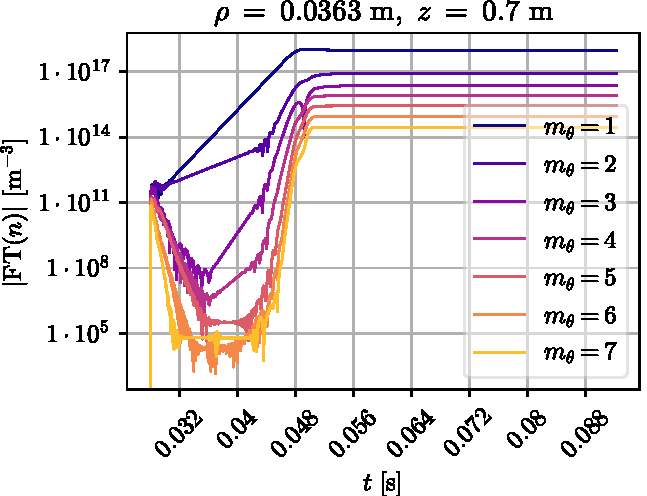
\includegraphics{fig/results/neutral/FFTnn1pct}
    \caption{Time trace of the absolute amplitude of the Fourier transformed density for $d=1\%$.}
    \label{fig:FFTnn1pct}
\end{figure}
%


\section{The saturated turbulence state}
%
As $d=1\%$ is not reaching a saturated steady state it will not be considered here.
The time trace of the parallel energy becomes more intermittent for decreasing ionization.
However, there are only minor changes in the radial direction.
The position of the fluctuations stays the same for all $d$, as shown in \cref{fig:nnScanPosOfFluct}.
%
\begin{figure}[htb]
    \centering
    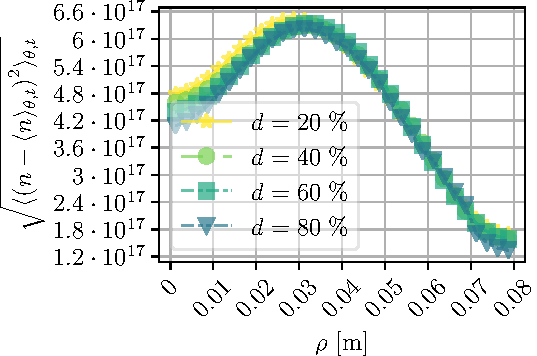
\includegraphics{fig/results/neutral/nnScanPosOfFluct}
    \caption{The standard deviation for the turbulent cases.}
    \label{fig:nnScanPosOfFluct}
\end{figure}
%
The skewness and kurtosis shows no general trend when changing $d$.
For the regions of low poloidal shear the skewness and kurtosis of $d=20\%$ and $d=40\%$ have approximately the same values for the skewness and the kurtosis.
Both the skewness and kurtosis increases in this region for $d=60\%$, before it approximately falls to the levels of $d=20\%$ for the $d=80\%$ case.
In the region of strong shear the intermittency increases for $d=20\%$, whereas it decreases for $d=80\%$.
%
\begin{figure}[htb]
    \centering
    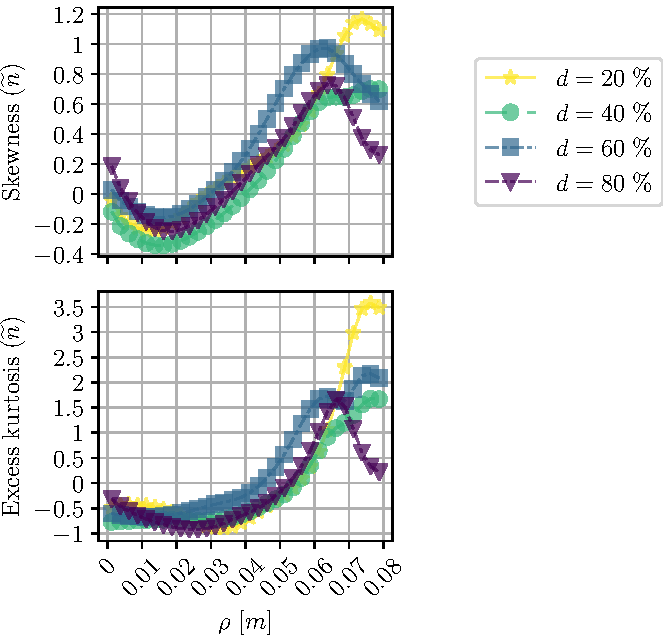
\includegraphics{fig/results/neutral/nnScanSkewKurt}
    \caption{The skewness and kurtosis for the turbulent cases.}
    \label{fig:nnScanSkewKurt}
\end{figure}
%

By looking at the flux in \cref{fig:flux008}, we can observe an increase in both the parallel and perpendicular flux for lower ionization degrees.
For the perpendicular case, this means that the radial turbulent transport is increasing.
%
\begin{figure}[htb]
    \centering
    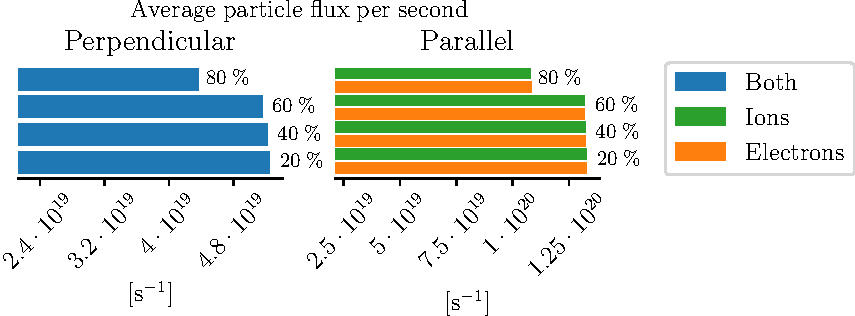
\includegraphics{fig/results/neutral/nnScanTotalFlux}
    \caption{
        The variation of the total flux as a function of $d$.
        The point of measurement is the same as in \cref{fig:flux008}.
    }
    \label{fig:nnScanTotalFlux}
\end{figure}
%

Finally, the average blob count presented in \cref{fig:nnScanBlobCount} reveals that the number of coherent structures increases with decreasing ionization level until $d=20\%$, where the blob and hole count is decreasing.
The decrease can be attributed to the overall decrease in growth in \cref{fig:grNn} together with more damping through the increased neutral resistivity.
%
\begin{figure}[htb]
    \centering
    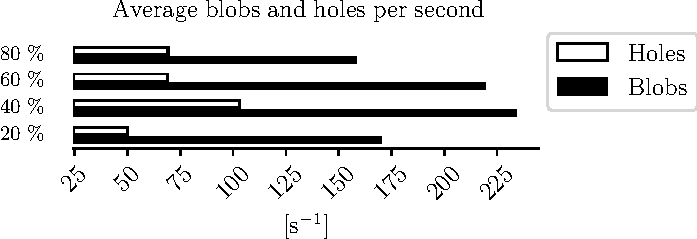
\includegraphics{fig/results/neutral/nnScanBlobCount}
    \caption{The blob count as a function of $d$ for a triggering signal of $3\sigma$ on the radial flux.}
    \label{fig:nnScanBlobCount}
\end{figure}
%
